% Created 2023-06-11 Sun 23:25
% Intended LaTeX compiler: pdflatex
\documentclass[11pt]{article}
\usepackage[utf8]{inputenc}
\usepackage[T1]{fontenc}
\usepackage{graphicx}
\usepackage{longtable}
\usepackage{wrapfig}
\usepackage{rotating}
\usepackage[normalem]{ulem}
\usepackage{amsmath}
\usepackage{amssymb}
\usepackage{capt-of}
\usepackage{hyperref}
\graphicspath{{../../books/}}
\usepackage{minted}
% TIPS
% \substack{a\\b} for multiple lines text





% pdfplots will load xolor automatically without option
\usepackage[dvipsnames]{xcolor}

\usepackage{forest}
% two-line text in node by [two \\ lines]
% \begin{forest} qtree, [..] \end{forest}
\forestset{
  qtree/.style={
    baseline,
    for tree={
      parent anchor=south,
      child anchor=north,
      align=center,
      inner sep=1pt,
    }}}
%\usepackage{flexisym}
% load order of mathtools and mathabx, otherwise conflict overbrace

\usepackage{mathtools}
%\usepackage{fourier}
\usepackage{pgfplots}
\usepackage{amsthm, mathabx,  amsmath, commath}
\usepackage{amsfonts}

\usepackage{empheq}
\usepackage{tikz}
\usetikzlibrary{arrows.meta}
\usepackage[most]{tcolorbox}

\newtheorem{theorem}{Theorem}[section]
\newtheorem{definition}{Definition}[section]
\newtheorem{corollary}{Corollary}[section]
\newtheorem{example}{Example}[section]
\newtheorem{lemma}{Lemma}[section]
\newtheorem{proposition}{Proposition}[section]

\newcommand{\bl}[1] {\boldsymbol{#1}}
\newcommand{\Wt}[1] {\stackrel{\sim}{\smash{#1}\rule{0pt}{1.1ex}}}
\newcommand{\wt}[1] {\widetilde{#1}}


%For boxed texts in align, use Aboxed{}
%otherwise use boxed{}

\DeclareMathSymbol{\widehatsym}{\mathord}{largesymbols}{"62}
\newcommand\lowerwidehatsym{%
  \text{\smash{\raisebox{-1.3ex}{%
    $\widehatsym$}}}}
\newcommand\fixwidehat[1]{%
  \mathchoice
    {\accentset{\displaystyle\lowerwidehatsym}{#1}}
    {\accentset{\textstyle\lowerwidehatsym}{#1}}
    {\accentset{\scriptstyle\lowerwidehatsym}{#1}}
    {\accentset{\scriptscriptstyle\lowerwidehatsym}{#1}}
}

\usepackage{graphicx}
    
% text on arrow for xRightarrow
\makeatletter
%\newcommand{\xRightarrow}[2][]{\ext@arrow 0359\Rightarrowfill@{#1}{#2}}
\makeatother


\def \bx {\boldsymbol{x}}
\def \ba {\boldsymbol{a}}
\def \bI {\boldsymbol{I}}
\def \bt {\boldsymbol{t}}
\def \bb {\boldsymbol{b}}
\def \bA {\boldsymbol{A}}
\def \bX {\boldsymbol{X}}
\def \bu {\boldsymbol{u}}
\def \bS {\boldsymbol{S}}
\def \bZ {\boldsymbol{Z}}
\def \bz {\boldsymbol{z}}
\def \by {\boldsymbol{y}}
\def \bw {\boldsymbol{w}}
\def \bT {\boldsymbol{T}}
\def \bS {\boldsymbol{S}}
\def \bm {\boldsymbol{m}}
\def \bW {\boldsymbol{W}}
\def \bY {\boldsymbol{Y}}
\def \bH {\boldsymbol{H}}
\def \blambda {\boldsymbol{\lambda}}
\def \bPhi {\boldsymbol{\Phi}}
\def \btheta {\boldsymbol{\theta}}
\def \bmu {\boldsymbol{\mu}}
\def \bphi {\boldsymbol{\phi}}
\def \bSigma {\boldsymbol{\Sigma}}
\def \lb {\left\{}
\def \rb {\right\}}
\def \caln {\mathcal{N}}
\def \dissum {\displaystyle\Sigma}
\def \dispro {\displaystyle\prod}
\def \E {\mathbb{E}}
\def \Q {\mathbb{Q}}
\def \V {\mathbb{V}}
\def \R {\mathbb{R}}
\def \calq {\mathcal{Q}}
\def \calg {\mathcal{G}}
\def \caln {\mathcal{N}}
\def \calr {\mathcal{R}}
\def \calm {\mathcal{M}}
\def \calc {\mathcal{C}}
\def \bcup {\bigcup}

\makeindex
\author{Tyler Akidau \& Slava Chernyak \& Reuven Lax}
\date{\today}
\title{Streaming Systems}
\hypersetup{
 pdfauthor={Tyler Akidau \& Slava Chernyak \& Reuven Lax},
 pdftitle={Streaming Systems},
 pdfkeywords={},
 pdfsubject={},
 pdfcreator={Emacs 29.0.90 (Org mode 9.6.1)}, 
 pdflang={English}}
\begin{document}

\maketitle
\tableofcontents


\section{Streaming 101}
\label{sec:org35a4e3f}
A type of data processing engine that is designed with infinite datasets in mind.

\begin{itemize}
\item Correctness: Streaming systems need a method for checkpointing persistent state over time.
\cite{akidau2013millwheel}, spark streaming: \cite{zaharia2013discretized}, flink snapshot:
\cite{carbone2015lightweight}
\item Tools for reasoning about time.
\end{itemize}

Event time: when events actually occurred

Processing time: when events are observed in the system
\begin{itemize}
\item shared resource limitations, like network congestion, network partition, shared CPU in a
nondedicated environment
\item software
\item features of the data
\end{itemize}

Fixed windows:
\begin{itemize}
\item Problem: network partition, events are collected globally and must be transferred to a common
location before processing, delaying processing until you’re sure all events have been
collected or reprocessing the entire batch for a given window whenever data arrive late
\end{itemize}


\begin{itemize}
\item Time-agnostic:
\begin{itemize}
\item filtering
\item inner joins
\end{itemize}
\item Approximation algorithms: top-n, k-means
\item windowing
\begin{center}
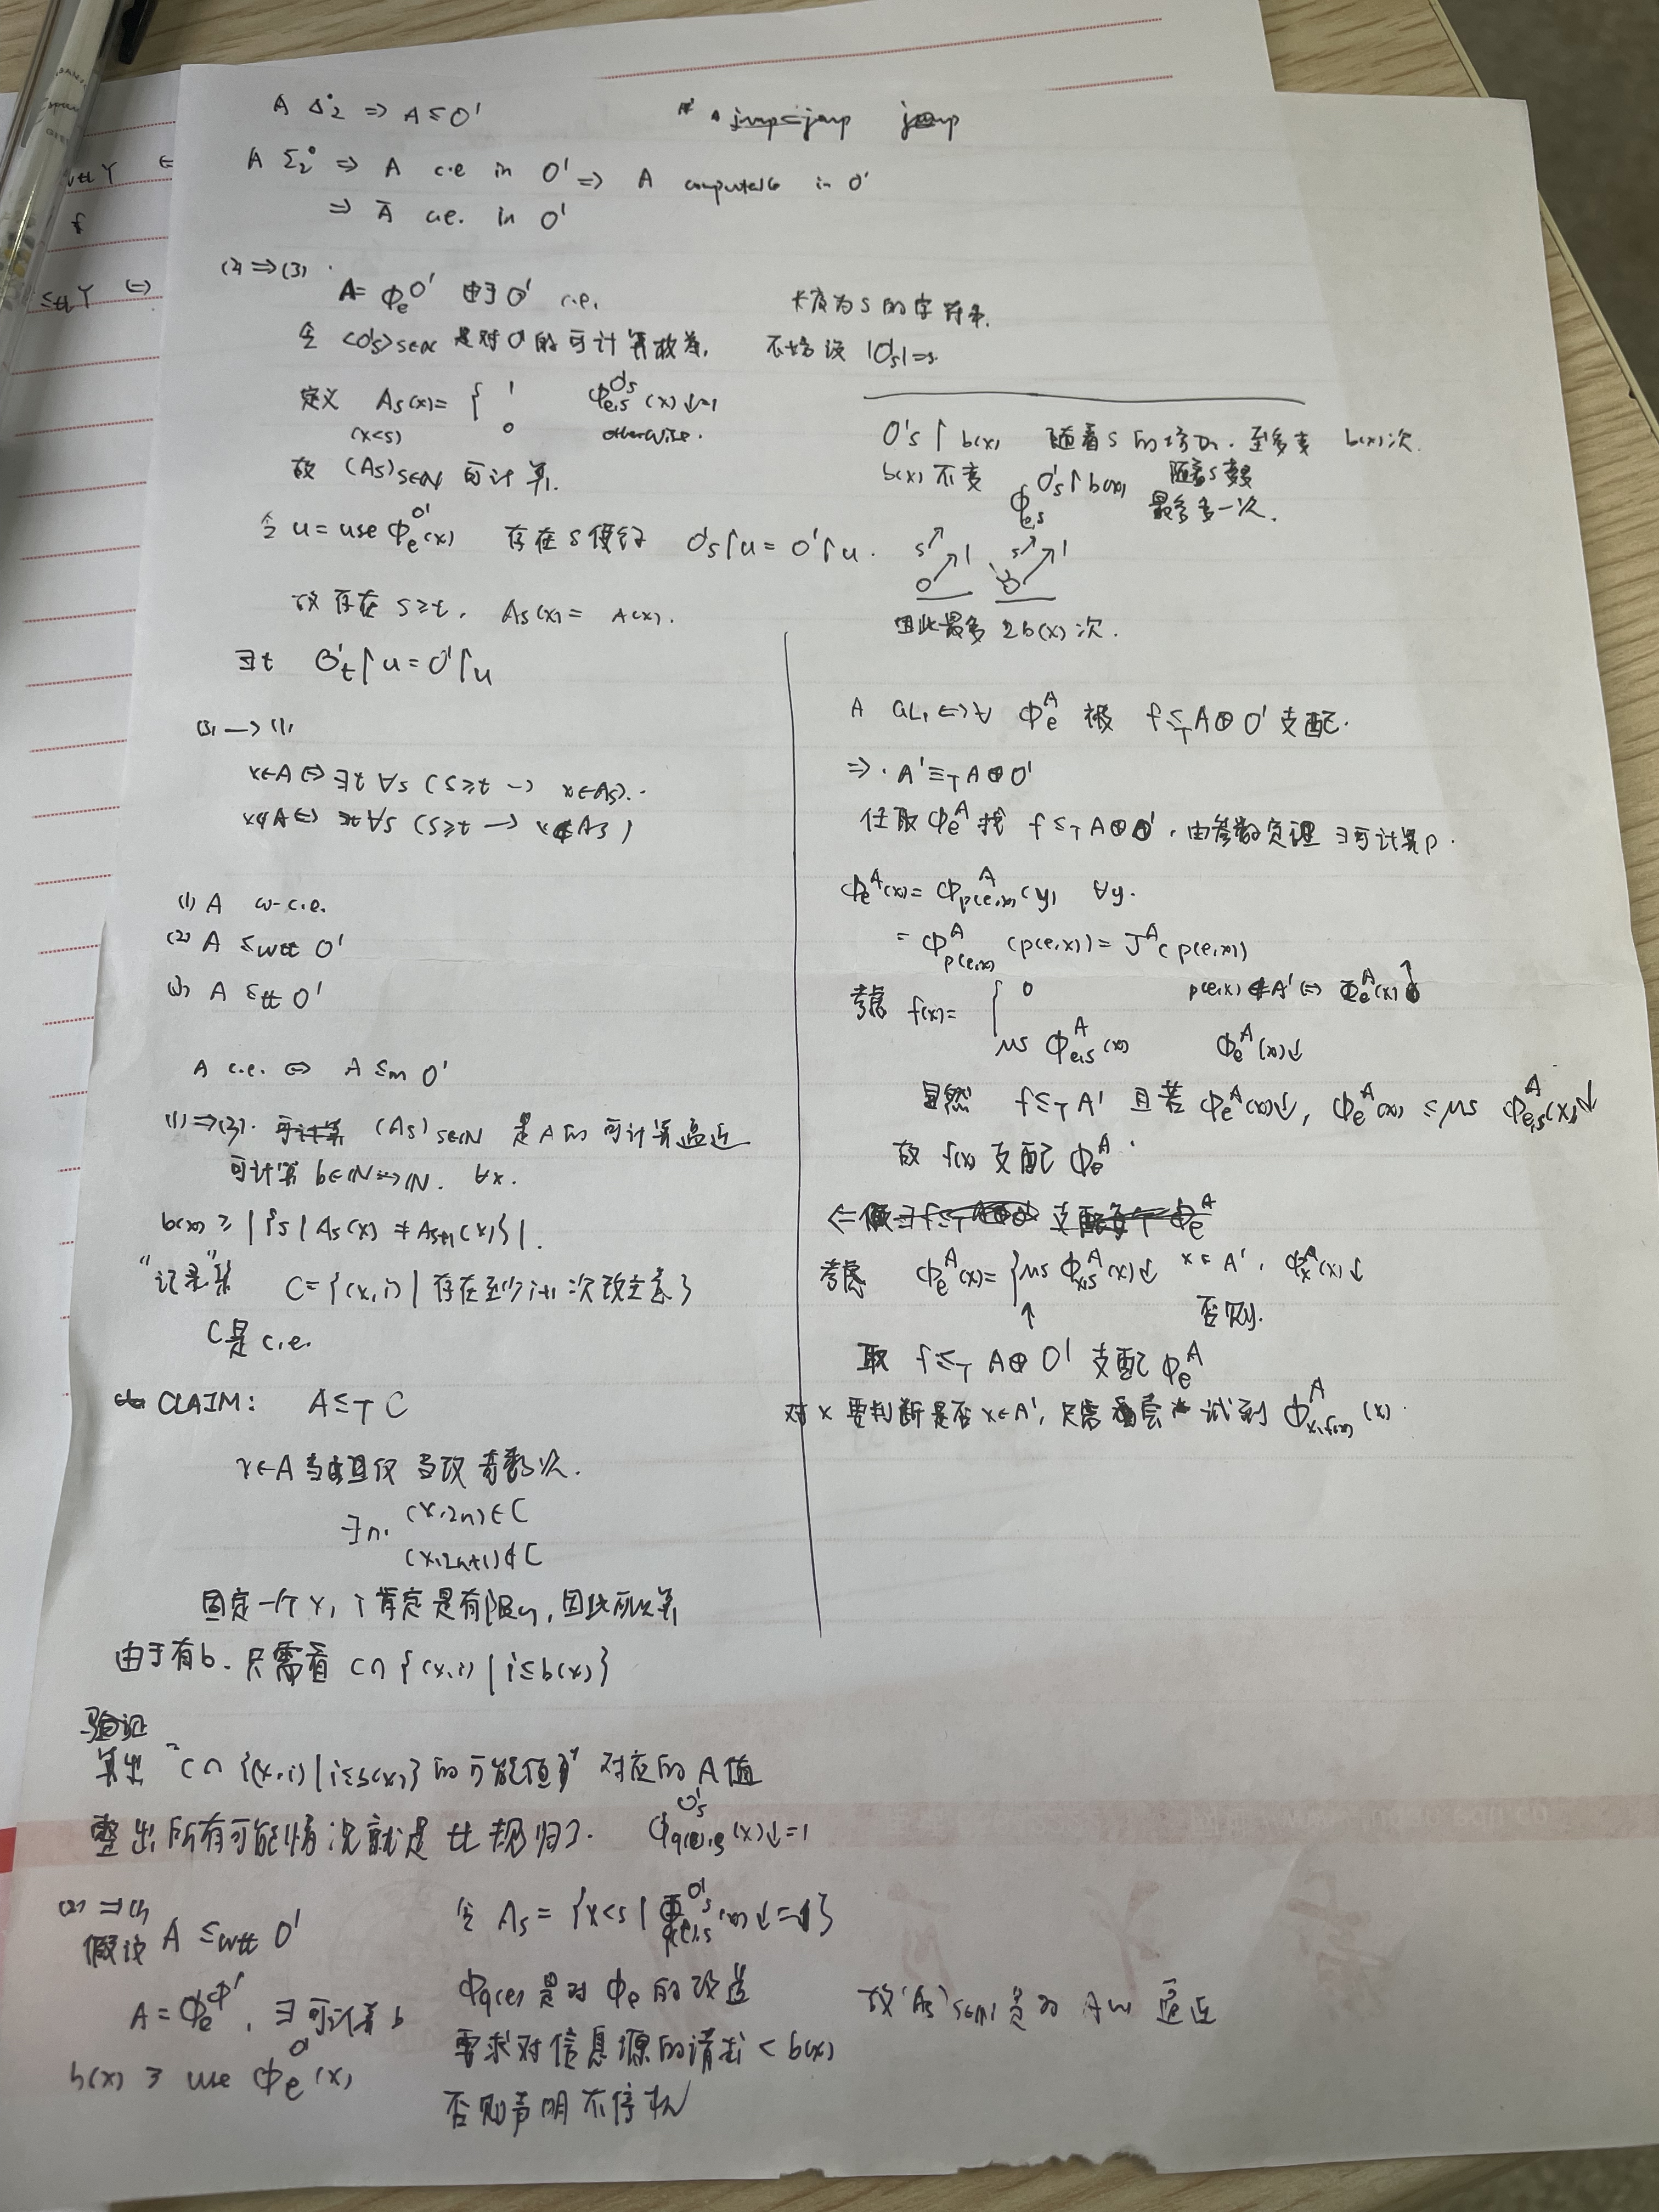
\includegraphics[width=.8\textwidth]{../images/streamingsystems/1.png}
\label{}
\end{center}
\begin{itemize}
\item Windowing by processing time: the system essentially buffers up incoming data into windows
until some amount of processing time has passed

Problem: if the data in question have event times associated with them, those data must
arrive in event-time order if the processing-time windows are to reflect the reality of when
those events actually happened.
\item windowing by event time
\end{itemize}
\end{itemize}

\section{The What, Where, When, and How of Data Processing}
\label{sec:orgad440ef}
\begin{itemize}
\item What results are calculated?
\item Where in event time are results calculated?
\item When in processing time are results materialized?
\item How do refinements of results relate?
\end{itemize}
\subsection{What: Transformations}
\label{sec:org57e5253}
In the rest of this chapter (and indeed, through much of the book), we look at a single example:
computing keyed integer sums over a simple dataset consisting of nine values.

\begin{center}
\begin{tabular}{llrrr}
\hline
Name & Team & Score & EventTime & ProcTime\\[0pt]
\hline
Julie & TeamX & 5 & 12:00:26 & 12:05:19\\[0pt]
Frank & TeamX & 9 & 12:01:26 & 12:08:19\\[0pt]
Ed & TeamX & 7 & 12:02:26 & 12:05:39\\[0pt]
Julie & TeamX & 8 & 12:03:06 & 12:07:06\\[0pt]
Amy & TeamX & 3 & 12:03:39 & 12:06:13\\[0pt]
Fred & TeamX & 4 & 12:04:19 & 12:06:39\\[0pt]
Naomi & TeamX & 3 & 12:06:39 & 12:07:19\\[0pt]
Becky & TeamX & 8 & 12:07:26 & 12:08:39\\[0pt]
Naomi & TeamX & 1 & 12:07:46 & 12:09:00\\[0pt]
\hline
\end{tabular}
\end{center}

In Beam:
\begin{itemize}
\item \texttt{PCollections}: datasets accoss which parallel transformations can be performed
\item \texttt{PTransforms}: applied to \texttt{PCollections} to create new \texttt{PCollections}.
\begin{center}
\includegraphics[width=.8\textwidth]{../images/streamingsystems/2.png}
\captionof{figure}{\label{}Types of transformations}
\end{center}
\end{itemize}
In our examples, we start out with a pre-loaded \texttt{PCollection<KV<Team,Integer>>} named ``input''
\begin{minted}[]{java}
PCollection<String> raw = IO.read(...);
PCollection<KV<Team, Integer>> input = raw.apply(new ParseFn());
PCollection<KV<Team, Integer>> totals =
input.apply(Sum.integersPerKey());
\end{minted}
For classical batch processing, it looks like \href{http://www.streamingbook.net/fig/2-3}{this}.
\subsection{Where: Windowing}
\label{sec:org5fe1c63}
\begin{minted}[]{java}
PCollection<KV<Team, Integer>> totals = input
    .apply(Window.into(FixedWindows.of(TWO_MINUTES)))
    .apply(Sum.integersPerKey());
\end{minted}

\href{http://www.streamingbook.net/fig/2-5}{result}

As before, inputs are accumulated in state until they are entirely consumed,
after which output is produced. In this case, however, instead of one output,
we get four: a single output, for each of the four relevant two-minute event-
time windows.
\subsection{Going Streaming: When and How}
\label{sec:orge6ce209}
\subsubsection{When: The Wonderful Thing About Triggers Is Triggers Are Wonderful Things}
\label{sec:org4112ddd}
Two types of triggers:
\begin{itemize}
\item \textbf{Repeated update triggers}: These periodically generate updated panes for a window as its
contents evolve. These updates can be materialized with every new record, or they can happen
after some processing-time delay, such as once a minute. The choice of period for a repeated
update trigger is primarily an exercise in balancing latency and cost.
\item \textbf{Completeness triggers}: These materialize a pane for a window only after the input for that
window is believed to be complete to some threshold. This type of trigger is most analogous to
what we’re familiar with in batch processing: only after the input is complete do we provide a
result. The difference in the trigger-based approach is that the notion of completeness is
scoped to the context of a single window, rather than always being bound to the completeness
of the entire input.
\end{itemize}
\begin{minted}[]{java}
PCollection<KV<Team, Integer>> totals = input
.apply(Window.into(FixedWindows.of(TWO_MINUTES))
.triggering(Repeatedly(AfterCount(1))));
.apply(Sum.integersPerKey());
\end{minted}
\href{http://www.streamingbook.net/fig/2-6}{result}

Two approaches for processing-time delays in triggers:
\begin{itemize}
\item \textbf{aligned delays}: the delay slices up processing time into fixed regions that align across keys
and windows
\item \textbf{unaligned delays}: the delay is relative to the data observed within a given window
\end{itemize}
\begin{minted}[]{java}
PCollection<KV<Team, Integer>> totals = input
    .apply(Window.into(FixedWindows.of(TWO_MINUTES))
                 .triggering(Repeatedly(AlignedDelay(TWO_MINUTES)))
    .apply(Sum.integersPerKey());
\end{minted}
\href{http://www.streamingbook.net/fig/2-7}{result}

The nice thing about it is predictability; you get regular updates across all modified windows
at the same time. That’s also the downside: all updates happen at once, which results in bursty
workloads that often require greater peak provisioning to properly handle the load.

\begin{listing}[H]
\caption{Triggering on unaligned two-minute processing-time boundaries}
\label{}
\begin{minted}[,frame=lines]{java}
PCollection<KV<Team, Integer>> totals = input
    .apply(Window.into(FixedWindows.of(TWO_MINUTES))
                 .triggering(Repeatedly(UnalignedDelay(TWO_MINUTES))
    .apply(Sum.integersPerKey());
\end{minted}
\end{listing}


\href{http://www.streamingbook.net/fig/2-8}{result}
\subsubsection{When: Watermarks}
\label{sec:org379ffeb}
Watermarks are a supporting aspect of the answer to the question: “When in processing time are
results materialized?” Watermarks are temporal notions of input completeness in the event-time
domain. Worded differently, they are the way the system measures progress and completeness
relative to the event times of the records being processed in a stream of events

\begin{center}
\includegraphics[width=.8\textwidth]{../images/streamingsystems/3.png}
\captionof{figure}{\label{}Event-time progress, skew, and watermarks}
\end{center}

We can think of the watermark as a function \(P\to F\) from processing time to event time. That
point in event time, \(E\), is the point up to which the system believes all inputs with event
times less than \(E\) have been observed.

Depending upon the type of watermark, perfect or heuristic, that assertion can be a strict
guarantee or an educated guess, respectively:
\begin{itemize}
\item \textbf{Perfect watermarks}: For the case in which we have perfect knowledge of all of the input data,
it’s possible to construct a perfect watermark.
\item \textbf{Heuristic watermarks}: use whatever information is available about the inputs (partitions,
ordering within partitions if any, growth rates of files, etc.) to provide an estimate of
progress that is as accurate as possible. In many cases, such watermarks can be remarkably
accurate in their predictions.
\end{itemize}

Because they provide a notion of completeness relative to our inputs, watermarks form the
foundation for the second type of trigger mentioned previously: \textbf{completeness triggers}.

\begin{listing}[H]
\caption{test}
\begin{minted}[]{c++}
awefawef
\end{minted}
\end{listing}
\section{Watermarks}
\label{sec:org050c69d}

\section{Advanced Windowing}
\label{sec:org90f653a}

\section{Exactly-Once and Side Effects}
\label{sec:org4571db9}

\section{Streams and Tables}
\label{sec:org584cd1e}

\section{The Practicalities of Persistent State}
\label{sec:org780623f}

\section{Streaming SQL}
\label{sec:org55645ca}

\section{Streaming Joins}
\label{sec:org677ab71}

\section{The Evolution of Large-Scale Data Processing}
\label{sec:org2e8c33f}
\end{document}